



\chapter{Formal Foundations}


This chapter describes the formal foundations of MayBMS, including the
principles used for representing and storing probabilistic data, the
design of the query language, and efficient algorithms for query processing.

It is safe for a reader who has gained sufficient intuitive understanding
of the workings of MayBMS from the tutorial to skip this chapter on
first reading and to directly proceed to the query language reference
chapter that follows.

%To do: Say what the reader should at least skim over (e.g., the abstract
%definition of probabilistic databases) and what she can skip in the first
%reading and which can be looked up for reference. We may ultimately want
%to move this chapter to the end of the manual or into the appendix in
%order not to discourage the readers too much.


\section{Probabilistic Databases: Notation}
\label{sect:probdb}
\index{Probabilistic database}


\def\ww{{\bf W}}


Given a schema with relation names $R_1, \dots, R_k$. We use $sch(R_l)$ to denote the attributes of relation schema $R_l$.
Formally, 
a {\em probabilistic database}\/ is a {\em finite}\/ set of structures
\[
\ww = \{ \tuple{R_1^1, \dots, R_k^1, p^{[1]}}, \dots,
         \tuple{R_1^n, \dots, R_k^n, p^{[n]}} \}
\]
of relations $R_1^i, \dots, R_k^i$ and numbers $0 < p^{[i]} \le 1$ such that
\[
\sum_{1 \le i \le n} p^{[i]} = 1.
\]
%
We call an element $\tuple{R_1^i, \dots, R_k^i, p^{[i]}} \in \ww$
a {\em possible world}\/, and $p^{[i]}$ its probability.
We use superscripts for indexing possible worlds.
To avoid confusion with exponentiation,
we sometimes use bracketed superscripts $\cdot^{[i]}$.
%
We call a relation $R$ {\em complete}\/ or {\em certain}\/
if its instantiations are the same in all possible worlds of $\ww$, i.e., if $R^1 = \cdots = R^n$.

Tuple {\em confidence}\/ refers to the probability of the event $\vec{t} \in R$, where $R$ is one of the relation names of the schema, with
\[
\Pr[\vec{t} \in R] = \sum_{1 \le i \le n:\; \vec{t} \in R^i} p^{[i]}.
\]









\section{Query Language Desiderata}
\label{sect:desiderata}
\index{Query language desiderata}


At the time of writing this, there is no accepted standard query language for probabilistic databases. In fact, we do not even agree today what use cases and functionality such systems should support.
It seems to be proper to start the query language discussion with the definition of design
{\em desiderata}\/. The following are those used in the design of MayBMS.
%
\begin{enumerate}
\item
Efficient query evaluation.

\item
The right degree of expressive power. The language should be powerful enough to support important queries. On the other hand, it should not be too strong, because expressiveness generally comes at a price: high evaluation complexity and infeasibility of query optimization.

\item
Genericity. The semantics of a query language should be independent from details of how the data is represented. Queries should behave in the same way no matter how the probabilistic data is stored. This is a basic requirement that is even part of the traditional definition of what constitutes a query (cf.\ e.g.\ \cite{AHV95}), but it is nontrivial to achieve for probabilistic databases \cite{AKO07ISQL}.

\item
The ability to transform data.
Queries on probabilistic databases are often interpreted quite narrowly in the literature.
%
%Probabilistic inference is sometimes understood as the problem of
%evaluating Boolean queries, or as ranking tuples by probability.
%
It is the authors' view that queries in general should be compositional mappings between databases, in this case probabilistic databases. This is a property taken for granted in relational databases. It allows for the definition of clean database update languages.

\item
The ability to introduce additional uncertainty.
This may appear to be a controversial goal, since uncertainty is commonly considered undesirable, and probabilistic databases are there to deal with it by providing useful functionality {\em despite}\/ uncertainty.
However, it can be argued that an uncertainty-introduction operation is important for at least three reasons:
(1)  for compositionality, and to allow construction of an uncertain database from scratch (as part of the update language);
(2) to support what-if queries; and
(3) to extend the hypothesis space modeled by the probabilistic database. The latter is needed to accommodate the results of experiments or new evidence, and to define queries that map from prior to posterior probabilistic databases. This is a nontrivial issue, and will be discussed in more detail later.
\end{enumerate}


The next section introduces a query algebra and argues that it satisfies each of these desiderata.









\section{The Algebra}
\label{sect:pwsa}
\index{Probabilistic world-set algebra}


This section covers the core query algebra of MayBMS: {\em probabilistic world-set algebra}\/ (probabilistic WSA) \cite{AKO07ISQL, Koch2008, Koch2008-SO}.
Informally, probabilistic world-set algebra consists of the operations of relational algebra,
an operation for computing tuple confidence conf, and the repair-key operation for {\em introducing}\/ uncertainty.
%
The operations of relational algebra are evaluated individually, in ``parallel'',
in each possible world.
The operation conf$(R)$
computes, for each tuple that occurs in relation $R$ in at least one world, the
sum of the probabilities of the worlds in which the tuple occurs.
The result is a certain relation, or viewed differently, a relation that is the same in
all possible worlds.
Finally, repair-key$_{\vec{A}@P}(R)$, where $\vec{A}, P$ are attributes of $R$,
conceptually nondeterministically chooses a maximal repair of
key $\vec{A}$.
This operation turns a possible world $R^i$ into the set of worlds consisting of all possible
{\em maximal repairs}\/ of key $\vec{A}$. A repair of key $\vec{A}$ in relation $R^i$ is a subset of $R^i$ for which $\vec{A}$ is a key.
It uses the numerically-valued column $P$ for weighting the newly created alternative
repairs.



Formally, probabilistic world-set algebra consists of the following operations:
\begin{itemize}
\item
The operations of relational algebra (selection $\sigma$, projection $\pi$,
product $\times$, union $\cup$, difference $-$, and attribute renaming $\rho$),
which are applied in each possible world independently.
\index{relational algebra}

The semantics of operations $\Theta$ on probabilistic database $\ww$ is
%
\[
\Bracks{\Theta(R_l)}(\ww) \; :=
\{ \tuple{R_1,\dots,R_k, \Theta(R_l), p}
\mid \tuple{R_1,\dots,R_k, p} \in \ww \}
\]
for unary operations ($1 \le l \le k$). For binary operations, the semantics is
\[
\Bracks{\Theta(R_l, R_m)}(\ww) \; :=
\{ \tuple{R_1,\dots,R_k, \Theta(R_l, R_m), p}
\mid \tuple{R_1,\dots,R_k, p} \in \ww \}.
\]

Selection conditions are Boolean combinations of atomic
conditions (i.e., negation is permitted even in the positive fragment of the algebra).
Arithmetic expressions may occur
in atomic conditions and in the arguments of $\pi$ and $\rho$. For example,
$\rho_{A+B \rightarrow C}(R)$ in each world
adds up the $A$ and $B$ values of each tuple
of $R$ and keeps them in a new $C$ attribute.



\item
An operation for computing tuple confidence,
\[
\Bracks{\mbox{conf}(R_l)}(\ww) :=
\{ \tuple{R_1,\dots,R_k, S, p} \mid \tuple{R_1,\dots,R_k, p} \in \ww \}
\]
where, w.l.o.g., $P \not\in sch(R_l)$, and
\[
S = \{ \tuple{\vec{t}, P: \Pr[\vec{t} \in R_l]} \mid
   \vec{t} \in \bigcup_i R_l^i \},
\]
with schema $sch(S) = sch(R_l) \cup \{ P \}$.
%
%Note that $S$ is a single certain relation with a
%column $P$ for holding probability values, rather than a probabilistic database.
%
The result of $\mbox{conf}(R_l)$, the relation $S$, is the same in all possible worlds, i.e., it is a certain relation.

By our definition of probabilistic databases, each possible world has nonzero probability. As a
consequence, conf does not return tuples with probability 0.

For example, on probabilistic database
\begin{center}
\begin{tabular}{c@{~~~}c@{~~~}c}
\begin{tabular}{@{~}c@{~}|@{~}c@{~~}c@{~}}
\hline
$R^{1}$ & A & B \\
\hline
& a & b \\
& b & c \\
\end{tabular}
$p^{[1]} = .3$
&
\begin{tabular}{@{~}c@{~}|@{~}c@{~~}c@{~}}
\hline
$R^{2}$ & A & B \\
\hline
& a & b \\
& c & d \\
\end{tabular}
$p^{[2]} = .2$
&
\begin{tabular}{@{~}c@{~}|@{~}c@{~~}c@{~}}
\hline
$R^{3}$ & A & B \\
\hline
& a & c \\
& c & d \\
\end{tabular}
$p^{[3]} = .5$
\end{tabular}
\end{center}
%
conf($R$) computes, for each possible tuple, the sum of the weights of the
possible worlds in which it occurs, here
%
\begin{center}
\begin{tabular}{c|c@{~~}c@{~~}c}
\hline
conf$(R)$ & $A$ & $B$ & P \\
\hline
& a & b & .5 \\
& a & c & .5 \\
& b & c & .3 \\
& c & d & .7 \\
\end{tabular}
\end{center}



\item
An uncertainty-introducing operation,
{\em repair-key}\/, which can be thought of as sampling a maximum repair of
a key for a relation.
Repairing a key of a complete relation $R$ means to compute, as possible worlds,
all subset-maximal relations
obtainable from $R$ by removing tuples such that a key constraint is satisfied.
We will use this as a method for constructing probabilistic databases,
with probabilities derived from relative weights attached to the tuples of $R$.
\index{Key repair}

We say that relation $R'$ is a {\em maximal repair}\/ of a functional dependency (fd, cf.\ \cite{AHV95}) for relation $R$ if $R'$ is a maximal subset of $R$ which satisfies that functional dependency, i.e., a subset $R' \subseteq R$ that satisfies the fd
such that there is no relation $R''$ with $R' \subset R'' \subseteq R$ that satisfies the fd.


Let $\vec{A}, B \in sch(R_l)$.
For each possible world $\tuple{R_1, \dots, R_k, p} \in \ww$,
let column $B$ of $R$ contain only numerical values greater than 0
and
let $R_l$ satisfy the fd $(sch(R_l) - B) \rightarrow sch(R_l)$.
Then,
\begin{multline*}
\Bracks{\rk_{\vec{A}@B}(R_l)}(\ww) \; := \\
\Big\{
\tuple{R_1, \dots, R_k, \pi_{sch(R_l)-B}(\hat{R}_l), \hat{p}}
\mid
\tuple{R_1, \dots, R_k, p} \in \ww,
\\
\mbox{$\hat{R}_l$ is a maximal repair of fd $\vec{A} \rightarrow sch(R_l)$},
\\
\hat{p} = p \cdot \prod_{\vec{t} \in \hat{R}_l}
  \frac{\vec{t}.B}
       {\sum_{\vec{s} \in R_l: \vec{s}.\vec{A}=\vec{t}.\vec{A}} \vec{s}.B}
\Big\}
\end{multline*}

Such a repair operation, apart from its usefulness for the purpose implicit
in its name, is a powerful way of constructing probabilistic databases from
complete relations.


\begin{example}\em
\label{ex:biased2}
Consider the example of tossing a biased coin twice. We start with a certain database
\begin{center}
\begin{tabular}{c|c@{~~}c@{~~}c}
\hline
R & Toss & Face & FProb \\
\hline
 & 1 & H & .4 \\
 & 1 & T & .6 \\
 & 2 & H & .4 \\
 & 2 & T & .6 \\
\end{tabular}
$p = 1$
\end{center}
that represents the possible outcomes of tossing the coin twice.
We turn this into a probabilistic database that represents this information using alternative possible worlds for the four outcomes using the query
$
S := \mbox{repair-key}_{\mathrm{Toss}@\mathrm{FProb}}(R).
$
The resulting possible worlds are
\begin{center}
\begin{tabular}{c|c@{~~}c}
\hline
$S^1$ & Toss & Face \\
\hline
 & 1 & H \\
 & 2 & H \\
\end{tabular}
%
\begin{tabular}{c|c@{~~}c}
\hline
$S^2$ & Toss & Face \\
\hline
 & 1 & H \\
 & 2 & T \\
\end{tabular}
\\[.7ex]
%
\begin{tabular}{c|c@{~~}c}
\hline
$S^3$ & Toss & Face \\
\hline
 & 1 & T \\
 & 2 & H \\
\end{tabular}
%
\begin{tabular}{c|c@{~~}c}
\hline
$S^4$ & Toss & Face \\
\hline
 & 1 & T \\
 & 2 & T \\
\end{tabular}
\end{center}
with probabilities
$p^{[1]} = p \cdot \frac{.4}{.4+.6} \cdot \frac{.4}{.4+.6} =
.16$, $p^{[2]}=p^{[3]}=.24$, and $p^{[4]}=.36$.
\punto
\end{example}
\end{itemize}

The fragment of probabilistic WSA which excludes the difference operation is called
{\em positive}\/ probabilistic WSA.


Computing possible and certain tuples is redundant with conf:
\begin{eqnarray*}
\mbox{poss}(R) &:=& 
\pi_{sch(R)}(\mbox{conf}(R))
\\
\mbox{cert}(R) &:=& \pi_{sch(R)}(\sigma_{P=1}(\mbox{conf}(R)))
\end{eqnarray*}

%We will now use our algebra to compute tables of conditional probabilities.


\begin{example}\em
\label{ex:twotosses}
A bag of coins contains two fair coins and one double-headed coin. We take one coin out of the bag but do not look at its two faces to determine its type (fair or double-headed) for certain. Instead we toss the coin twice to collect evidence about its type.


\begin{figure}
\begin{center}
\begin{tabular}{@{~}c|c@{~}c@{~}}
\hline
Coins & Type & Count \\
\hline
 & fair         & 2 \\
 & 2headed & 1 \\
\\
\end{tabular}
\hspace{2mm}
\begin{tabular}{@{~}c|ccc@{~}}
\hline
Faces & Type & Face & FProb \\
\hline
 & fair    & H & .5 \\
 & fair    & T & .5 \\
 & 2headed & H &  1 \\
\end{tabular}
\hspace{2mm}
\begin{tabular}{@{~}c|c@{~}}
\hline
Tosses & Toss \\
\hline
 & 1 \\
 & 2 \\
\\
\end{tabular}

\medskip

\begin{tabular}{c|c}
\hline
$R^f$ & Type \\
\hline
 & fair          \\
\end{tabular}
\hspace{2mm}
\begin{tabular}{c|c}
\hline
$R^{dh}$ & Type \\
\hline
 & 2headed \\
\end{tabular}
%
\nop{
Corresponding U-RDB:
\begin{tabular}{c|cc|c}
\hline
$U_R$ & V & D & Type \\
\hline
 & c & fair    & fair      \\
 & c & 2headed & 2headed \\
\end{tabular}
%
\hspace{2mm}
%
\begin{tabular}{c|ccc}
\hline
$W$ & V & D & P \\
\hline
 & c & fair    & $2/3$ \\
 & c & 2headed & $1/3$ \\
\end{tabular}
} % end nop

\medskip

\nop{
\begin{tabular}{c@{~}|@{~}c@{~~}c@{~~}c@{~~}c}
\hline
$S^f$ & Face & FProb & Toss \\
\hline
 & H & .5 & 1 \\
 & T & .5 & 1 \\
 & H & .5 & 2 \\
 & T & .5 & 2 \\
\end{tabular}
\hspace{2mm}
\begin{tabular}{c@{~}|@{~}c@{~~}c@{~~}c@{~~}c}
\hline
$S^{dh}$ & Face & FProb & Toss \\
\hline
 & H &  1 & 1 \\
 & H &  1 & 2 \\
\end{tabular}

\begin{tabular}{@{~}c@{~}|@{~}c@{~~}c@{~}|@{~}c@{~~}c@{~~}c@{~~}c@{~}}
\hline
$U_S$ & V & D & Face & FProb & Toss \\
\hline
 & c & fair    & H & .5 & 1 \\
 & c & fair    & T & .5 & 1 \\
 & c & fair    & H & .5 & 2 \\
 & c & fair    & T & .5 & 2 \\
 & c & 2headed & H &  1 & 1 \\
 & c & 2headed & H &  1 & 2 \\
\end{tabular}
\begin{tabular}{@{~}c@{~}|@{~}c@{~~}c@{~~}c@{~}}
\hline
$W$ & V & D & P \\
\hline
 & c & fair    & $2/3$ \\
 & c & 2headed & $1/3$ \\
\end{tabular}
} % end nop




\nop{
\begin{tabular}{@{~}c@{~}|@{~}c@{~~}c@{~~}c@{~~}c@{~}|@{~}c@{~~}c@{~}}
\hline
$U_T$ & $V_1$ & $D_1$ & $V_2$ & $D_2$ & Toss & Face \\
\hline
 & c & fair      & f.1  & H & 1 & H \\
 & c & fair      & f.1  & T & 1 & T \\
 & c & fair      & f.2  & H & 2 & H \\
 & c & fair      & f.2  & T & 2 & T \\
 & c & 2headed   & 2h.1 & H & 1 & H \\
 & c & 2headed   & 2h.2 & H & 2 & H \\
\end{tabular}
\hspace{0.5mm}
\begin{tabular}{@{~}c@{~}|@{~}c@{~~}c@{~~}c@{~}}
\hline
$W$ & V & D & P \\
\hline
 & c    & fair      & $2/3$ \\
 & c    & 2headed   & $1/3$ \\
 & f.1  & H         & .5 \\
 & f.1  & T         & .5 \\
 & f.2  & H         & .5 \\
 & f.2  & T         & .5 \\
 & 2h.1 & H         & 1 \\
 & 2h.2 & H         & 1 \\
\end{tabular}

Now there are five possible worlds.
} % end nop



\begin{tabular}{ccc}
\begin{tabular}{@{~}c@{~}|@{~}c@{~}c@{~~}c@{~}}
\hline
$S^{f.HH}$ & Type & Toss & Face \\
\hline
& fair & 1 & H \\
& fair & 2 & H \\
\end{tabular}
&
\begin{tabular}{@{~}c@{~}|@{~}c@{~}c@{~~}c@{~}}
\hline
$S^{f.HT}$ & Type & Toss & Face \\
\hline
& fair & 1 & H \\
& fair & 2 & T \\
\end{tabular}
&
\begin{tabular}{@{~}c@{~}|@{~}c@{~}c@{~~}c@{~}}
\hline
$S^{dh}$ & Type & Toss & Face \\
\hline
& 2headed & 1 & H \\
& 2headed & 2 & H \\
\end{tabular}
\\
$p^{f.HH}=1/6$ & $p^{f.HT}=1/6$ & $p^{dh}=1/3$
\\[1ex]
\begin{tabular}{@{~}c@{~}|@{~}c@{~}c@{~~}c@{~}}
\hline
$S^{f.TH}$ & Type & Toss & Face \\
\hline
& fair & 1 & T \\
& fair & 2 & H \\
\end{tabular}
&
\begin{tabular}{@{~}c@{~}|@{~}c@{~}c@{~~}c@{~}}
\hline
$S^{f.TT}$ & Type & Toss & Face \\
\hline
& fair & 1 & T \\
& fair & 2 & T \\
\end{tabular}
&
\\
$p^{f.TH}=1/6$ & $p^{f.TT}=1/6$ &
\end{tabular}

\medskip

\begin{tabular}{@{~}c@{~}|@{~}c@{~~}c@{~}}
\hline
Ev & Toss & Face \\
\hline
 & 1 & H \\
 & 2 & H \\
\end{tabular}
\hspace{2mm}
\begin{tabular}{c@{~}|@{~}c@{~~}c}
\hline
$Q$ & Type & P \\
\hline
 & fair    & $(1/6)/(1/2) = 1/3$ \\
 & 2headed & $(1/3)/(1/2) = 2/3$ \\
\end{tabular}
\end{center}

\caption{Tables of Example~\ref{ex:twotosses}.}
\label{fig:twotosses_tables}
\end{figure}


We start out with a complete database (i.e., a relational database, or a probabilistic database with one possible world of probability 1) consisting of
three relations, Coins, Faces, and Tosses (see Figure~\ref{fig:twotosses_tables} for all tables used in this example).
%
We first pick a coin from the bag and model that
the coin be either fair or double-headed.
In probabilistic WSA this is expressed as
\[
R := \mbox{repair-key}_{\emptyset@\mathrm{Count}}(\mathrm{Coins}).
\]

This results in a probabilistic database of two possible worlds,
\[
\{ \tuple{\mbox{Coins}, \mbox{Faces}, R^f, p^{f}=2/3},
   \tuple{\mbox{Coins}, \mbox{Faces}, R^{dh}, p^{dh}=1/3} \}.
\]

The possible outcomes of tossing the coin twice can be modeled as
\[
S := \mbox{repair-key}_{\mathrm{Toss@FProb}}(
   R \bowtie \mathrm{Faces} \times \mathrm{Tosses}).
\]
This turns the two possible worlds into five, since there are four possible outcomes of tossing the fair coin twice, and only one for the double-headed coin.

Let $T := \pi_{\mathrm{Toss}, \mathrm{Face}}(S)$.
The posterior probability
that a coin of type $x$ was picked, given the {\em evidence}\/ $Ev$ (see Figure~\ref{fig:twotosses_tables}) that both tosses result in
H, is
\[
\Pr[x \in R \mid T = Ev] = \frac{\Pr[x \in R \land T = Ev]}{\Pr[T=Ev]}.
\]
Let $A$ be a relational algebra expression for the Boolean query $T=Ev$.
Then we can compute a table of pairs
$\tuple{x, \Pr[x \in R \mid T = Ev]}$ as
\[
Q := \pi_{\mathrm{Type}, P_1/P_2 \rightarrow P}(\rho_{P \rightarrow P_1}(\mbox{conf}(R \times A)) \times \rho_{P \rightarrow P_2}(\mbox{conf}(A))).
\]

The prior probability that the chosen coin was fair was 2/3; after taking the
evidence from two coin tosses into account, the posterior probability
$\Pr$[the coin is fair $|$ both tosses result in H] is only 1/3.
Given the evidence from the coin tosses, the coin is now more likely to be double-headed.
\punto
\end{example}


\begin{example}\em
\label{ex:2}
%
We redefine the query of Example~\ref{ex:twotosses} such that
repair-key is only applied to certain relations.
Starting from the database obtained by computing $R$, with its two possible worlds, we perform the query
$
S_0 := \mbox{repair-key}_{\mathrm{Type,Toss@FProb}}
      (\mathrm{Faces} \times \mathrm{Tosses})
$
to model the possible outcomes of tossing the chosen coin twice.
%
The probabilistic database representing these repairs consists of
eight possible worlds, with the two possible $R$ relations of Example~\ref{ex:twotosses} and, independently, four possible $S_0$ relations.
%
\nop{
$
\tuple{\mbox{Coins}, \mbox{Faces}, R^{ct \in \{f, dh\}}, S_0^j, p^{ct}/4},
$
with the four possible relations $S^j_0$
%
\begin{center}
\begin{tabular}{cc}
\begin{tabular}{@{~}c@{~}|@{~}c@{~~}c@{~~}c@{~~}c@{~}}
\hline
$S_0^1$ & Type & Toss & Face \\
\hline
& fair     &  1   & H \\
& fair     &  2   & H \\
& 2headed  &  1   & H \\
& 2headed  &  2   & H \\
\end{tabular}
&
\begin{tabular}{@{~}c@{~}|@{~}c@{~~}c@{~~}c@{~~}c@{~}}
\hline
$S_0^2$ & Type & Toss & Face \\
\hline
& fair     &  1   & T \\
& fair     &  2   & H \\
& 2headed  &  1   & H \\
& 2headed  &  2   & H \\
\end{tabular}
\\[2ex]
\\
\begin{tabular}{@{~}c@{~}|@{~}c@{~~}c@{~~}c@{~~}c@{~}}
\hline
$S_0^3$ & Type & Toss & Face \\
\hline
& fair     &  1   & H \\
& fair     &  2   & T \\
& 2headed  &  1   & H \\
& 2headed  &  2   & H \\
\end{tabular}
&
\begin{tabular}{@{~}c@{~}|@{~}c@{~~}c@{~~}c@{~~}c@{~}}
\hline
$S_0^4$ & Type & Toss & Face \\
\hline
& fair     &  1   & T \\
& fair     &  2   & T \\
& 2headed  &  1   & H \\
& 2headed  &  2   & H \\
\end{tabular}
\end{tabular}
\end{center}
%
For instance, the world with relations $R^{f}$ and $S_0^1$ has probability $2/3 \cdot 1/4 = 1/6$.
} % end nop
%
Let $S := R \bowtie S_0$.
While we now have eight possible worlds rather than five, the four worlds in which the double-headed coin was picked
all agree on $S$ with the one world in which the double-headed coin was picked in Example~\ref{ex:twotosses}, and the sum of their probabilities is the same as the probability of that world.
It follows that the new definition of $S$ is equivalent to the one of
Example~\ref{ex:twotosses} and the rest of the query is the same.
%
% and the new definition of $S$ can be used interchangeably with
% the one from Example~\ref{ex:twotosses}.
\punto
\end{example}




\paragraph{Discussion}
%
The repair-key operation admits an interesting class of queries:
Like in Example~\ref{ex:twotosses}, we can start with a probabilistic database of prior probabilities, add further evidence (in Example~\ref{ex:twotosses}, the result of
the coin tosses) and then compute interesting posterior probabilities. The adding of further
evidence may require extending the hypothesis space first. For this, the repair-key operation is
essential. Even though our goal is not to update the database, we have to be able to introduce uncertainty just to be able to model new evidence -- say, experimental data.
Many natural and important probabilistic database queries cannot be expressed without the repair-key operation. The coin tossing example was admittedly a toy example (though hopefully easy to understand). Real applications such as diagnosis or processing scientific data involve technically similar questions.

Regarding our desiderata, it is quite straightforward to see that probabilistic WSA is generic (3):
see also the proof for the non-probabilistic language in \cite{AKO07ISQL}. It is clearly a data transformation query language (4) that supports powerful queries for defining databases. The repair-key operation is our construct for uncertainty introduction (5). The evaluation efficiency (1) of probabilistic WSA is studied in Section~\ref{sect:theory}. Expressiveness (2) is best demonstrated by the ability of a language to satisfy many relevant use cases. While there are no agreed upon expressiveness benchmarks for probabilistic databases yet, this manual provides numerous examples that are closely related to natural use cases.






\section{Representing Probabilistic Data}
\label{sect:representation}


This section discusses the method used for representing and storing probabilistic
data and correlations in MayBMS.
We start by motivating the problem of finding a practical representation system.


\begin{example}\em
\label{ex:census}
Consider a census scenario, in which a large number of individuals manually fill in forms.
The data in these forms subsequently has to be put into a database, but no matter whether this is done automatically using OCR or by hand, some uncertainty may remain about the correct values for some of the answers. Below are two simple filled in forms. Each one contains the
social security number, name, and marital status of one person.

\begin{center}
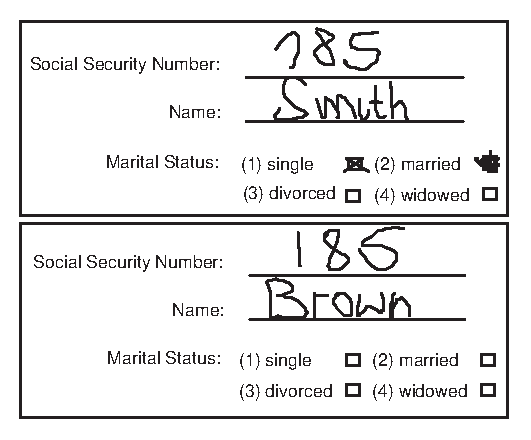
\epsfig{width=6cm,file=census.eps}
\end{center}

The first person, Smith, seems to have checked marital status ``single'' after first mistakenly checking ``married'', but it could also be the opposite.
%
%, if the user wanted to point out the correct answer by filling the box.
%
The second person, Brown, did not answer the marital status question.
The social security numbers also have several possible readings. Smith's could be 185 or 785 (depending on whether Smith originally is from the US or from Europe) and Brown's may either be 185 or 186.

In an SQL database, uncertainty can be managed using null values, using a table
\begin{center}
\begin{tabular}{c|ccc}
\hline
(TID) & SSN & N & M \\
\hline
$t_1$ & null & Smith & null \\
$t_2$ & null & Brown & null \\
\end{tabular}
\end{center}

Using nulls, information is lost about the values considered possible for the various fields. Moreover, it is not possible to express correlations such as that, while social security numbers may be uncertain, no two distinct individuals can have the same. In this example, we can exclude the case that both Smith and Brown have social security number 185.
Finally, we cannot store probabilities for the various alternative possible worlds.
\punto
\end{example}


This leads to three natural desiderata for a representation system:
(*) Expressiveness, that is, the power to represent all (relevant) probabilistic databases,
(*) succinctness, that is, space-efficient storage of the uncertain data,
and (*) efficient real-world query processing.

Often there are many rather (but not quite) independent
local alternatives in probabilistic data, which multiply up to a very large number of possible worlds.
For example, the US census consists of many dozens of questions for about 300 million individuals.
Suppose forms are digitized using OCR and the resulting data contains just
two possible readings for 0.1\% of the answers before cleaning.
Then, there are on the order of $2^{10,000,000}$ possible worlds, and each one will take
close to one Terabyte of data to store. 
Clearly, we need a way of representing this data that is much better than a naive enumeration of possible worlds.

Also, the repair-key operator of probabilistic world-set algebra in general causes an exponential increase in the number of possible worlds.

There is a trade-off between succinctness on one hand and efficient processing on the other.
Computing confidence conf$(Q)$ of conjunctive queries $Q$ on tuple-independent databases
is \#P-hard -- one such hard query \cite{dalvi07efficient} (in datalog notation \cite{AHV95}) is
\[
Q \leftarrow R(x), S(x,y), T(y).
\]
At the same time, much more expressive queries can be evaluated efficiently on nonsuccinct representations (enumerations of possible worlds) \cite{AKO07ISQL}. Query evaluation in probabilistic databases is not hard because of the presence of probabilities, but because of the succinct storage of alternative possible worlds!
We can still have the goal of doing well in practice.


\paragraph{Conditional tables}
\index{C-tables}
MayBMS uses a purely relational representation system for probabilistic databases called {\em U-relational databases}\/, which is based
on probabilistic versions of the classical {\em conditional tables}\/ (c-tables) of the database literature \cite{IL1984}.
Conditional tables are a relational representation system based on the notion of {\em labeled null values}\/ or {\em variables}\/, that is, null values that have a name. The name makes it possible to use the same variable $x$ in several fields of a database, indicating that the value of $x$ is unknown but must be the same in all those fields in which $x$ occurs. Tables with variables are also known as {\em v-tables}\/.


Formally, c-tables are v-tables extended by a column for holding a local condition. That is, each tuple of a c-table has a Boolean condition constructed using ``and'', ``or'', and ``not'' from atomic conditions of the form $x = c$ or $x = y$, where $c$ are constants and $x$ and $y$ are {\em variables}\/.
Possible worlds are determined by functions $\theta$ that map each variable that occurs in at least one of the tuples or local conditions in the c-tables of the database to a constant. The database in that possible world is obtained by (1) selecting those tuples whose local condition $\phi$ satisfies the variable assignment $\theta$, i.e., that becomes true if each variable $x$ in $\phi$ is replaced by $\theta(x)$, (2) replacing all variables $y$ in the value fields of these tuples by $\theta(y)$, and (3) projecting away the local condition column. For example, the following c-table represents the possible
worlds for the census forms:

\begin{center}
	\begin{tabular}{c|c|c|c|c}
		\hline
		R & SSN & N & M & cond\\\hline
		  & 185 & Smith & y & $x = 1$\\
		  & 785 & Smith & y & $x = 2$\\
		  & 785 & Smith & y & $x = 3$\\
		  & 186 & Brown & z & $x = 1$\\
		  & 185 & Brown & z & $x = 2$\\
		  & 186 & Brown & z & $x = 3$\\
	\end{tabular}
\end{center}

The variables $y$ and $z$ have domains $\{1,2\}$ and $\{1,2,3,4\}$, respectively and encode the marital statuses of the two persons, and variable
$x$ with domain $\{1,2,3\}$ is used to encode the uniqueness of the social security constraint. Indeed, under any valuation $\theta$ the tuples having social security status of 185 do not have their local conditions satisfied at the same time.

Conditional tables are sometimes defined to include a notion of {\em global condition}\/, which
we do not use: We want each probabilistic database to have at least one possible world. We can encode the same information as above using the following c-table with global condition $\Phi = (u\neq v)$, where $u: dom(u) = \{185,785\}, v: dom(v) = \{185,186\}$ are the variables holding the social security numbers:

\begin{center}
	\begin{tabular}{c|c|c|c|c}
		\hline
		R & SSN & N & M & cond\\\hline
		  & u & Smith & y & true \\
		  & v & Brown & z & true \\
	\end{tabular}
\end{center}


Conditional tables are a so-called {\em strong representation system}\/: They are closed under the application of relational algebra queries. The set of worlds obtained by evaluating a relational algebra query in each possible world represented by a conditional table can again be straightforwardly represented by a conditional table. Moreover, the local conditions are in a sense the most natural and simple formalism possible to represent the result of queries on data with labeled nulls.
%The local conditions just represent the information necessary to preserve correctness and can also be understood to be just data provenance information \cite{BSHW2006}.

%For nonprobabilistic uncertain databases, c-tables are the {\em gold standard}\/ that any
%formalism for representing uncertain data {\em and}\/ supporting relational algebra
%query processing should be measured against.


\paragraph{U-Relational Databases}
%
In our model, probabilistic databases are finite sets of possible worlds with probability weights. It follows that each variable naturally has a finite domain, the set of values it can take across all possible worlds. This has several consequences.
%
First, variables can be considered {\em finite random variables}\/.
Second, only allowing for variables to occur in local conditions,
but not in attribute fields of the tuples,
means no restriction of expressiveness.
Moreover, we may assume without loss of generality that each atomic condition is of the form $x=c$ (i.e., we never have to compare variables).

If we start with a c-table in which each local condition is a conjunction of no more than $k$ atomic conditions, then a positive relational algebra query on this uncertain database will result in a c-table in which each local condition is a conjunction of no more than $k'$ atoms, where $k'$ only depends on $k$ and the query, but not on the data. If $k$ is small, it is reasonable to actually hard-wire it in the schema, and represent local conditions by $k$ pairs of columns to store atoms of the form $x=c$.

These are the main ideas of our representation system, U-relations.
Random variables are assumed independent in the {\em current}\/ MayBMS system, but as we will see, this means no restriction of generality.
Nevertheless, it is one goal of future work to support
graphical models for representing more correlated joint probability distributions below our U-relations. This would allow us to represent {\em learned}\/ distributions in the form of e.g.\ Bayesian networks directly in the system (without the need to map them to local conditions) and run queries on top, representing the inferred correlations using local conditions. The latter seem to be better suited for representing the incremental correlations constructed by queries.

One further idea employed in U-relational databases is to use vertical partitioning for representing {\em attribute-level uncertainty}\/, i.e., to allow to decompose tuples in case several fields of a tuple are independently uncertain.


\begin{example}\em
\label{ex:urelation}
The following set of tables is a U-relational database representation for the census data scenario
of Example~\ref{ex:census}, extended by suitable probabilities for the various alternative values the fields can take (represented by table $W$).
%
\begin{center}
\begin{tabular}{c}
\begin{tabular}{l|cc|c|c}
\hline
$U_{R[SSN]}$ & V & D & TID & SSN \\
\hline
& $x$ & $1$ & $t_1$ & 185 \\
& $x$ & $2$ & $t_1$ & 785 \\
& $y$ & $1$ & $t_2$ & 185 \\
& $y$ & $2$ & $t_2$ & 186 \\
\end{tabular}
\\[15mm]
\begin{tabular}{l|cc|c|c}
\hline
$U_{R[M]}$ & V & D & TID & M \\
\hline
& $v$ & $1$ & $t_1$ & 1 \\
& $v$ & $2$ & $t_1$ & 2 \\
& $w$ & $1$ & $t_2$ & 1 \\
& $w$ & $2$ & $t_2$ & 2 \\
& $w$ & $3$ & $t_2$ & 3 \\
& $w$ & $4$ & $t_2$ & 4 \\
\end{tabular}
\end{tabular}
%
\hspace{5mm}
%
\begin{tabular}{c}
\begin{tabular}{l|c|c}
\hline
$U_{R[N]}$ & TID & N \\
\hline
      & $t_1$ & Smith \\
      & $t_2$ & Brown \\
\end{tabular}
\\[10mm]
\begin{tabular}{l|cc|l}
\hline
$W$ & V & D & P \\
\hline
& $x$ & $1$ & .4 \\
& $x$ & $2$ & .6 \\[.8ex]
& $y$ & $1$ & .7 \\
& $y$ & $2$ & .3 \\[.8ex]
& $v$ & $1$ & .8 \\
& $v$ & $2$ & .2 \\[.8ex]
& $w$ & $1$ & .25 \\
& $w$ & $2$ & .25 \\
& $w$ & $3$ & .25 \\
& $w$ & $4$ & .25 \\
\end{tabular}
\end{tabular}
\end{center}
%\punto
\end{example}


\index{U-relation}
Formally, a U-relational database consists of a
set of independent random variables with finite domains (here, $x,y,v,w$),
a set of U-relations, and a ternary table $W$ (the {\em world-table}\/) for representing distributions. The $W$ table stores, for each variable, which values it can take and with what probability.
%
The schema of each U-relation consists of
a {\em set}\/ of pairs ($V_i, D_i$) of {\em condition columns}\/ representing variable assignments and a set of {\em value columns}\/ for representing the data values of tuples.

The semantics of U-relational databases is as follows.
Each possible world is identified by a valuation $\theta$ that assigns one
of the possible values to each variable.
The probability of the possible world is the product of weights of the
values of the variables.
A tuple of a U-relation, stripped of its condition columns, is in a given possible
world if its variable assignments are consistent with $\theta$.
Attribute-level uncertainty is achieved through \cby{vertical decompositioning}, so one of the value columns is used for storing tuple ids and undoing the vertical decomposition on demand.


\begin{example}\em
Consider the U-relational database of Example~\ref{ex:urelation} and
the possible world
\[
\theta = \{ x \mapsto 1, y \mapsto 2, v \mapsto 1, w \mapsto 1 \}.
\]
The probability weight of this world is $.4 \cdot .3 \cdot .8 \cdot .25 = .024$. By removing all the tuples
whose condition columns are inconsistent with $\theta$ and projecting away the condition columns,
we obtain the relations
\begin{center}
\begin{tabular}{l|l|l}
\hline
$R[SSN]$ & TID & SSN \\
\hline
& $t_1$ & 185 \\
& $t_2$ & 186 \\
\end{tabular}
%
\hspace{3mm}
%
\begin{tabular}{l|l|l}
\hline
$R[M]$ & TID & M \\
\hline
& $t_1$ & 1 \\
& $t_2$ & 1 \\
\end{tabular}
%
\hspace{3mm}
%
\begin{tabular}{l|l|l}
\hline
$R[N]$ & TID & N \\
\hline
      & $t_1$ & Smith \\
      & $t_2$ & Brown \\
\end{tabular}
\end{center}
which are just a vertically decomposed version of $R$ in the chosen possible world.
That is, $R$ is $R[SSN] \bowtie R[M] \bowtie R[N]$ in that possible world.
\punto
\end{example}


\paragraph{Properties of U-relations}
U-relational databases are a {\em complete}\/ representation system for (finite) probabilistic databases \cite{AJKO2008}. This means that any probabilistic database can be represented in this formalism. In particular, it follows that U-relations are closed under query evaluation using any generic query language, i.e., starting from a represented database, the query result can again be represented as a U-relational database.
Completeness also implies that any (finite) correlation structure among tuples can be represented, despite the fact that we currently assume that the random variables that our correlations are constructed from (using tuple conditions) are independent: The intuition that some form of graphical model for finite distributions may be more powerful (i.e., able to represent distributions that cannot be represented by U-relations) is {\em false}\/.


\nop{
\paragraph{Historical Note}
The first prototype of MayBMS \cite{AKO07WSD, AKO07WSDb, OKA2008} did not use U-relations for representations, but a different representation system called {\em world-set decompositions}\/
\cite{AKO07WSD}. These representations are based on factorizations of the space of possible worlds. They can also be thought of as shallow Bayesian networks.
The problem with this approach is that some selection operations can cause an exponential blowup of the representations. This problem is not shared by U-relations, even though they are strictly more succinct than world-set decompositions.
This was the reason for introducing U-relations in \cite{AJKO2008} and developing a new prototype of MayBMS based on U-relations.
} % end nop




\section{Conceptual Evaluation and Rewritings}
\label{sect:theory}


This section gives a complete solution for efficiently evaluating a large fragment of probabilistic world-set algebra using relational database technology. Then we discuss the evaluation of the remaining operations of probabilistic WSA, namely difference and tuple confidence. Finally, an overview of known worst-case computational complexity results is given.


\paragraph{Translating queries down to the representation relations}
Let $\textit{rep}$ be the {\em representation function}\/, which
maps a U-relational data\-base to the set of possible worlds it represents.
Our goal is to give a reduction that maps 
any positive relational algebra query $Q$ over probabilistic databases represented as U-relational
databases \textit{T} to an equivalent positive relational algebra query
$\overline{Q}$ of polynomial size such that
\[
\textit{rep}(\overline{Q}(T)) =
   \{Q({\cal A}^i) \mid {\cal A}^i \in \textit{rep}(T)\}
\]
where the ${\cal A}^i$ are relational database instances (possible worlds)
or, as a commutative diagram,
\vspace*{1em}
  \begin{center}
 \begin{psmatrix}[colsep=8em,rowsep=5em,nodesepA=3pt,nodesepB=3pt]
   $T$                                & $\overline{Q}(T)$\\
   $\{{\cal A}^1,\ldots,{\cal A}^n\}$ & 
   $\{Q({\cal A}^1),\ldots,Q({\cal A}^n)\}$
 %
   \ncline{->}{1,1}{2,1}<{\textit{rep}}
   \ncline{->}{2,1}{2,2}^{$Q$}
   \ncline{->}{1,1}{1,2}^{$\overline{Q}$}
   \ncline{->}{1,2}{2,2}>{\textit{rep}}
 \end{psmatrix}
  \end{center}


The following is such a reduction, which maps the
operations of positive relational algebra, poss, and repair-key
to relational algebra over U-relational representations:
\begin{eqnarray*}
\Bracks{R \times S} &:=&
  \pi_{(U_R.\overline{VD} \cup U_S.\overline{VD}) \rightarrow \overline{VD}, sch(R), sch(S)}( \\
&& \quad U_R \bowtie_{U_R.\overline{VD} \,\mathrm{consistent \, with}\, U_S.\overline{VD}} U_S)
\\
\Bracks{\sigma_\phi R} &:=& \sigma_\phi(U_R)
\\
\Bracks{\pi_{\vec{B}} R} &:=& \pi_{\overline{VD}, \vec{B}}(R)
\\
\Bracks{R \cup S} &:=& U_R \cup U_S
\\
\Bracks{\mbox{poss}(R)} &:=& \pi_{sch(R)}(U_R).
\end{eqnarray*}
The consistency test for conditions can be expressed simply using Boolean conditions (see Example~\ref{ex:proc_urel}, and \cite{AJKO2008}).
Note that the product operation, applied to two U-relations of $k$ and $l$ $(V_i, D_i)$ column pairs, respectively, returns a U-relation with $k+l$ $(V_i, D_i)$ column pairs.

For simplicity, let us assume that the elements of $\pi_{\tuple{\vec{A}}}(U_R)$ are not yet used
as variable names. Moreover, let us assume that the $B$ value column of $U_R$, which is to provide weights for the alternative values of the columns $sch(R) - (\vec{A} \cup B)$ for each tuple $\vec{a}$ in
$\pi_{\tuple{\vec{A}}}(U_R)$, are probabilities, i.e., sum up to one for each $\vec{a}$ and do not first have to be normalized as described in the definition of the semantics of repair-key in Section~\ref{sect:pwsa}.
The operation $S := \mbox{repair-key}_{\vec{A}@B}(R)$ for complete relation $R$ is translated as
\[
U_S := \pi_{\tuple{\vec{A}} \rightarrow V, \tuple{(sch(R)-\vec{A}) - \{B\}} \rightarrow D, sch(R)} U_R
\]
with
\[
W := W \cup \pi_{\tuple{\vec{A}} \rightarrow V,
                 \tuple{(sch(R) - \vec{A}) - \{B\}} \rightarrow D,
                 B \rightarrow P} U_R.
\]
Here, $\tuple{\cdot}$ turns tuples of values into atomic values that can be
stored in single fields.

That is, repair-key starting from a complete relation is just a
projection/copying of columns, even though we may create an
exponential number of possible worlds.

%Of course, we have to assure that the variables we introduce are new, but this is easy to do
%by concatenating the $\vec{A}$ values with a number generated using e.g.\ a logical clock or
%database sequence object.


\begin{example}\em
Consider again the relation $R$ of Example~\ref{ex:biased2}, which represents information about tossing a biased coin twice, and the query
%
$S := \mbox{repair-key}_{\mathrm{Toss}@\mathrm{FProb}}(R)$.
The result is
%
\begin{center}
\begin{tabular}{c|cc|ccc}
\hline
$U_S$ & V & D & Toss & Face & FProb \\
\hline
 & 1 & H & 1 & H & .4 \\
 & 1 & T & 1 & T & .6 \\
 & 2 & H & 2 & H & .4 \\
 & 2 & T & 2 & T & .6 \\
\end{tabular}
\hspace{5mm}
\begin{tabular}{c|ccc}
\hline
$W$ & V & D & P \\
\hline
 & 1 & H & .4 \\
 & 1 & T & .6 \\
 & 2 & H & .4 \\
 & 2 & T & .6 \\
\end{tabular}
\end{center}
as a U-relational database.
\punto
\end{example}


The projection technique only works if the relation that repair-key is applied to is certain.
However, this means no loss of generality (cf.\ \cite{Koch2008-SO}, and see also Example~\ref{ex:2}).

The next example demonstrates the application of the rewrite rules to compile a query down to relational algebra on the U-relations.


\begin{example}\em
\label{ex:proc_urel}
We revisit our census example with U-relations $U_{R[SSN]}$ and $U_{R[N]}$.
We ask for possible names of persons who have SSN 185,
\[
\mbox{poss}(\pi_N(\sigma_{SSN=185}(R))).
\]
To undo the vertical partitioning, the query
is evaluated as
\[
\mbox{poss}(\pi_N(\sigma_{SSN=185}(R[SSN] \bowtie R[N]))).
\]
We rewrite the query using our rewrite rules into 
\[
\pi_N(\sigma_{SSN=185}(U_{R[SSN]}
   \bowtie_{\psi\wedge\phi} U_{R[N]})),
\]
where
$\psi$ ensures that we only generate tuples that occur in some worlds,
\[
\psi := (U_{R[SSN]}.V = U_{R[N]}.V \Rightarrow
    U_{R[SSN]}.D=U_{R[N]}.D),
\]
and $\phi$ ensures that the vertical partitioning is correctly undone,
\[
\phi := (U_{R[SSN]}.TID = U_{R[N]}.TID).
\]

\vspace{-5mm}

\punto
\end{example}



\paragraph{Properties of the relational-algebra reduction}
The relational algebra rewriting down to positive relational algebra on U-relations has
a number of nice properties. First, since relational algebra has PTIME (even AC$_0$) data complexity, the query language of positive relational algebra, repair-key, and poss on probabilistic databases represented by U-relations has the same.
The rewriting is in fact a {\em parsimonious translation}\/: The number of algebra operations does not increase and each of the operations selection, projection, join, and union remains of the same kind. Query plans are hardly more complicated than
the input queries. As a consequence, we were able to observe that off-the-shelf relational database query optimizers
do well in practice \cite{AJKO2008}.



\section{Asymptotic Efficiency}


We have seen in the previous section that for all but two operations of
probabilistic world-set algebra, there is a very efficient
solution that builds on relational database technology.
These remaining operations are confidence computation and relational
algebra difference.


\paragraph{Approximate confidence computation}
\index{Confidence approximation}
%
To compute the confidence in a tuple of data values occurring possibly in several tuples
of a U-relation, we have to compute the probability of the disjunction of the local conditions of all these tuples. We have to eliminate duplicate tuples because we are interested in the  probability of the data tuples rather than some abstract notion of tuple identity that is really an artifact of our representation. That is, we have to compute the probability of a
DNF, i.e., the sum of the weights of the worlds identified with valuations $\theta$ of the random variables such that the DNF becomes true under $\theta$. This problem is \#P-complete
\cite{GGH1998,dalvi07efficient}. The result is not the sum of the probabilities of the individual conjunctive local conditions, because they may, intuitively, ``overlap''. 

\begin{example}\em
Consider
a U-relation with schema $\{V,D\}$ (representing a nullary relation) and two tuples 
$\tuple{x,1}$, and $\tuple{y,1}$, with the $W$ relation from Example~\ref{ex:urelation}.
Then the confidence in the nullary tuple $\tuple{}$ is $\Pr[x \mapsto 1 \lor y \mapsto 1] =
\Pr[x \mapsto 1] + \Pr[y \mapsto 1] - \Pr[x \mapsto 1 \land y \mapsto 1] = .82$.
\punto
\end{example}


Confidence computation can be efficiently approximated by Monte Carlo simulation \cite{GGH1998,dalvi07efficient,Koch2008}.
The technique is based on the Karp-Luby fully poly\-no\-mi\-al-time randomized approximation scheme (FPRAS) for counting the number of solutions to a DNF formula \cite{KL1983,KLM1989,DKLR2000}.
%
There is an efficiently computable unbiased estimator that in expectation returns the probability $p$ of a DNF of $n$ clauses (i.e., the local condition tuples of a Boolean U-relation) such that computing the average of a polynomial number of such Monte Carlo steps (= calls to the Karp-Luby unbiased estimator) is an $(\epsilon, \delta)$-approximation for the probability: If the average $\hat{p}$ is taken over at least $\lceil 3 \cdot n \cdot \log(2/\delta)/\epsilon^2 \rceil$ Monte Carlo steps, then $\Pr\big[ |p - \hat{p}| \ge \epsilon \cdot p \big] \le \delta$. The paper \cite{DKLR2000} improves upon this  by determining smaller numbers (within a constant factor from optimal) of necessary iterations to achieve an $(\epsilon, \delta)$-approximation.



%The assert operation is an update operation - a knowledge compilation operation --
%that modifies the database; In queries, assert can be replaced by computing conditional
%confidences, which can again be efficiently approximated.



\paragraph{Avoiding the difference operation}
%
Difference $R-S$ is conceptually simple on c-tables.
Without loss of generality, assume that $S$ does not contain tuples
$\tuple{\vec{a}, \psi_1}, \dots, \tuple{\vec{a}, \psi_n}$ that are duplicates if the local conditions are disregarded. (Otherwise, we replace them
by $\tuple{\vec{a}, \psi_1 \lor \dots \lor \psi_n}$.)
For each tuple $\tuple{\vec{a}, \phi}$ of $R$, if
$\tuple{\vec{a}, \psi}$ is in $S$ then output
$\tuple{\vec{a}, \phi \land \neg \psi}$; otherwise, output
$\tuple{\vec{a}, \phi}$.
Testing whether a tuple is possible in the result of a query involving difference is already NP-hard \cite{AKG1991}. For U-relations, we in addition have to turn $\phi \land \neg \psi$
into a DNF to represent the result as a U-relation.
This may lead to an exponentially large output and a very large number of $\vec{V}\vec{D}$ columns may be required to represent the conditions.
For these reasons, MayBMS currently does not implement the difference operation.

In many practical applications, the difference operation can be avoided.
Difference is only hard on uncertain relations. On such relations, it can only lead to displayable query results in queries that close the possible worlds semantics using conf, computing a single certain relation. 
%
Probably the most important application of the difference operation is for encoding universal constraints, for example in data cleaning.
But if the confidence operation is applied on top of a universal query, there is a trick that will often allow to rewrite the query into an
existential one  (which can be expressed in positive relational algebra plus conf,
without difference) \cite{Koch2008}.


\begin{example}\em
\label{ex:trick}
%
% BUG-FIX BEGIN
The example uses the census scenario and the uncertain relation $R[SSN]$
with columns TID and SSS discussed earlier; below we will call this relation
just simply $R$.
% BUG-FIX END
Consider the query of finding, for each TID $t_i$ and SSN $s$, the confidence in the statement that $s$ is the correct SSN for the individual associated with the tuple identified by $t_i$, assuming
that social security numbers uniquely identify individuals, that is, assuming that the functional dependency
$SSN \rightarrow TID$ (subsequently called $\psi$) holds.
In other words, the query asks, for each TID $t_i$ and SSN $s$, to find the probability $\Pr[\phi \mid \psi]$, where
$
\phi(t_i,s) = \exists t \in R\; t.TID=t_i \land t.SSN=s.
$
%
Constraint $\psi$ can be thought of as a data cleaning constraint that ensures that the SSN fields in no two distinct census forms (belonging to two different individuals) are interpreted as the same number. 

We compute the desired conditional probabilities, for each possible pair of a TID and an SSN, as
$
\Pr[\phi \mid \psi] = \Pr[\phi \land \psi] / \Pr[\psi].
$
Here $\phi$ is existential (expressible in positive relational algebra) and $\psi$ is an equality-generating dependency (i.e., a special universal query) \cite{AHV95}.
%
The trick is to turn relational difference into the subtraction of probabilities,
$\Pr[\phi \land \psi] = \Pr[\phi] - \Pr[\phi \land \neg \psi]$ and
$\Pr[\psi] = 1 - \Pr[\neg \psi]$, where
$
\neg \psi = \exists t,t' \in R \; t.SSN = t'.SSN \land t.TID \neq t'.TID
$
is existential (with inequalities). Thus $\neg \psi$ and $\phi \land \neg \psi$ are
expressible in positive relational algebra. This works for a considerable superset of the equality-generating dependencies \cite{Koch2008}, which in turn subsume useful data cleaning constraints.

Let $R_{\neg \psi}$ be the relational algebra expression for $\neg \psi$,
\[
\pi_\emptyset(R
   \bowtie_{TID=TID' \land SSN \neq SSN'}
   \rho_{TID \rightarrow TID'; SSN \rightarrow SSN'}(R)),
\]
and let $S$ be
% BUG-FIX BEGIN
\begin{multline*}
\rho_{P \rightarrow P_\phi}(\mbox{conf}(R)) \bowtie
\rho_{P \rightarrow P_{\phi \land \neg \psi}}
\big(
\mbox{conf}(R \times R_{\neg \psi})
\; \cup \\
\pi_{TID, SSN, 0 \rightarrow P}
(\mbox{conf}(R) - \mbox{conf}(R \times R_{\neg \psi}))
\big)
\times
\rho_{P \rightarrow P_{\neg \psi}}(\mbox{conf}(R_{\neg \psi})).
\end{multline*}
% BUG-FIX END
The overall example query can be expressed as
\[
T :=
\pi_{TID, SSN, (P_\phi - P_{\phi \land \neg \psi})/(1 - P_{\neg \psi}) \rightarrow P}(S).
\]
For the example table $R$ given above, $S$ and $T$ are
\begin{center}
\begin{tabular}{l|lllll}
\hline
$S$ & TID & SSN & $P_\phi$ & $P_{\phi \land \neg \psi}$ & $P_{\neg \psi}$ \\
\hline
& $t_1$ & 185 & .4 & .28 & .28 \\
& $t_1$ & 785 & .6 & 0   & .28 \\
& $t_2$ & 185 & .7 & .28 & .28 \\
& $t_2$ & 186 & .3 & 0   & .28 \\
\end{tabular}
\hspace{5mm}
\begin{tabular}{l|lll}
\hline
$T$ & TID & SSN & P \\
\hline
& $t_1$ & 185 & 1/6 \\
& $t_1$ & 785 & 5/6 \\
& $t_2$ & 185 & 7/12 \\
& $t_2$ & 186 & 5/12 \\
\end{tabular}
\end{center}
\end{example}



\paragraph{Complexity Overview}
\index{Complexity}
%
Figure~\ref{tab:complexity} gives an overview over the known complexity results for the various fragments of probabilistic WSA.


\begin{figure}
\begin{center}
\begin{tabular}{|l|l|}
\hline
Language Fragment & Complexity \\
\hline
\hline
Pos.RA + repair-key + possible &
{\bf in AC0}
\\[.3ex]
RA + possible & {\bf co-NP-hard}
\\[.3ex]
Conjunctive queries + conf & {\bf \#P-hard}
\\[.3ex]
Probabilistic WSA & {\bf in ${\mathbf P^{\#P}}$}
\\[.5ex]
Pos.RA + repair-key + possible &
\\
+ approx.conf + egds &  {\bf in PTIME}
\\
\hline
\end{tabular}
\end{center}
%
\caption{Complexity results for (probabilistic) world-set algebra
\cite{KochBook2008}.
RA denotes relational algebra.}
\label{tab:complexity}
\end{figure}


Difference \cite{AKG1991} and confidence computation \cite{dalvi07efficient} independently make queries NP-hard.
Full probabilistic world-set algebra is essentially not harder than the language of \cite{dalvi07efficient}, even though it is substantially more expressive.

It is worth noting that repair-key by itself, despite the blowup of possible worlds, does not make queries hard. For the language consisting of positive relational algebra, repair-key, and poss, we have shown by construction that it has PTIME complexity: We have given a positive relational algebra rewriting to queries on the representations earlier in this section. Thus queries are even in the highly parallelizable complexity class AC$_0$.

The final result in Figure~\ref{tab:complexity} concerns the language consisting of the positive relational algebra operations, repair-key, $(\epsilon, \delta)$-approximation of confidence computation, and the generalized equality generating dependencies of \cite{Koch2008} for which we can rewrite difference of uncertain relations to difference of confidence values (see Example~\ref{ex:trick}). The result is that queries of that language that close the possible worlds semantics -- i.e., that use conf to compute a certain relation -- are in PTIME overall.








